
\begin{minipage}{6.5cm}
	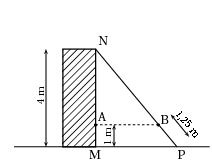
\includegraphics[scale=1]{TR-214.png} 
\end{minipage}
\begin{minipage}{11cm}
	\begin{enumerate}
		\item Calcule la distance $MP$ entre le pied du mur et le pied de l'échelle.
		\item L'inclinaison de l'échelle par rapport au sol horizontal est la mesure de l'angle $\widehat{MPN}$. Détermine la valeur, arrondie au degré, de cette mesure.
		\item Afin que l'échelle ne glisse pas sur le sol, on tend une corde entre un anneau $A$ situé à 1~m de hauteur sur le mur, et un barreau $B$ de l'échelle situé à 1,25~m du bas de l'échelle (voir figure).
		\begin{enumerate}
			\item Calcule $NA$ et $NB$.
			\item La corde est-elle parallèle au sol ?
		\end{enumerate}
	\end{enumerate}
\end{minipage}